\chapter{Kinetika Elektrode dan Elektroanalisis}\label{ch:b3:electrode-kinetics}

Setetes darah pada sebuah strip plastik, lima detik, sebuah angka: alat
pengukur glukosa yang dipakai jutaan orang beberapa kali sehari adalah sebuah
sel elektrokimia, dan yang diukurnya bukan tegangan melainkan arus. Sebuah
\omterm{def:b3:complex-kinetics:enzyme}{enzim} mengoksidasi glukosa, sebuah kompleks besi terlarut membawa
elektron-elektronnya ke elektrode karbon, dan arus yang mengalir ditentukan
oleh seberapa cepat kompleks itu berdifusi ke elektrode, jadi oleh
konsentrasinya. Bab ini menjelaskan mengapa elektron melintasi sebuah antarmuka
dengan cepat atau lambat (\omterm{thm:b3:electrode-kinetics:butler-volmer}{persamaan Butler--Volmer}), bagaimana transpor massa
membatasi arus, dan bagaimana \omterm{def:b3:electrode-kinetics:cv}{voltametri siklik} dan metode-metode
elektroanalisis lainnya mengubah arus menjadi konsentrasi, tetapan laju, dan
mekanisme.

\begin{recall}
Jilid Tahun 1 mendefinisikan potensial elektrode, potensial standar, persamaan
Nernst, elektrode acuan, dan setengah sel. Jilid Tahun 2 memperkenalkan kurva
arus--potensial dengan arus anodik dan arus katodiknya, elektrode kerja dan
elektrode lawan, overpotensial, sistem cepat dan sistem lambat, lapisan difusi
dan arus pembatas; koefisien aktivitas dan kekuatan ion; kurva kalibrasi,
metode adisi standar, dan batas deteksi. \Cref{ch:b3:rate-theories} memberikan
\omterm{def:b3:rate-theories:tst}{teori keadaan transisi}. Dari fisika: hukum-hukum difusi Fick, persamaan
Poisson, dan kapasitor.
\end{recall}

\begin{omfigure}
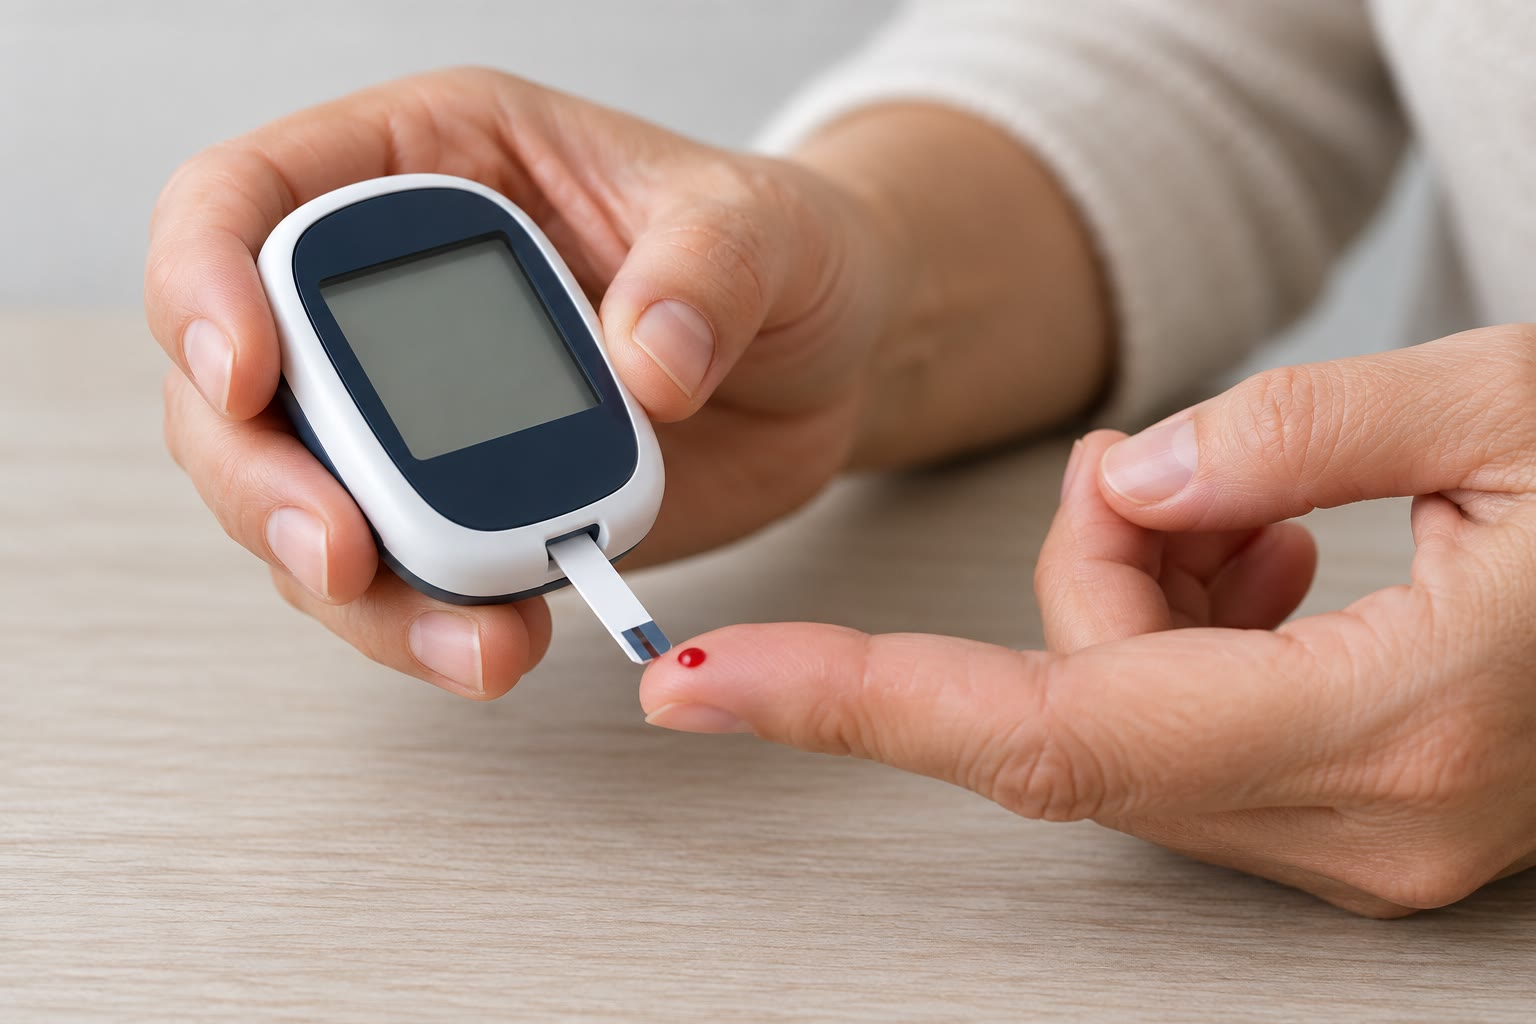
\includegraphics[width=0.6\linewidth]{images/book4/ai/b3-15-glucose-meter.jpg}

{\small Alat pengukur glukosa darah: stripnya membawa sel tiga elektrode yang
mungil dengan sebuah \omterm{def:b3:complex-kinetics:enzyme}{enzim} dan sebuah mediator redoks; alat itu memberikan
sebuah potensial dan membaca arusnya.}
\end{omfigure}

\section{Antarmuka elektrode--larutan}

Logam yang dicelupkan ke dalam larutan elektrolit membawa muatan permukaan,
dan larutan menjawabnya dengan muatan yang sama besar dan berlawanan tanda,
yang terdiri atas kelebihan ion-ion bertanda tertentu. Kedua lapisan muatan itu
membentuk kapasitor setebal ukuran molekul.

\begin{definition}[Lapisan rangkap listrik]\label{def:b3:electrode-kinetics:double-layer}
Yang disebut \emph{lapisan rangkap listrik}\index{lapisan rangkap listrik}
adalah susunan muatan pada antarmuka elektrode--larutan: muatan pada logam dan
muatan ion pengimbangnya dalam larutan. Bagian kompaknya, yang disebut
\emph{lapisan Helmholtz}\index{lapisan Helmholtz}, adalah lapisan ion dan
molekul pelarut yang bersentuhan dengan permukaan; sedangkan \emph{lapisan
difus}\index{lapisan difus} adalah daerah di luarnya, tempat gerak termal
menyebarkan ion-ion yang berlebih sejauh jarak yang berorde \emph{panjang
Debye}\index{panjang Debye} $\kappa^{-1}$. Yang disebut \emph{kapasitansi
lapisan rangkap}\index{kapasitansi lapisan rangkap} $C_{\mathrm{dl}}$ adalah
muatan yang tersimpan per satuan luas per volt potensial di seberang
antarmuka itu.
\end{definition}

\begin{proposition}[Panjang Debye]\label{prop:b3:electrode-kinetics:debye-length}
Dalam larutan dengan kekuatan ion $I$ (dalam \unit{mol.m^{-3}}) dan permitivitas
relatif $\varepsilon_r$, potensial kecil $\varphi_0$ pada elektrode meluruh ke dalam
larutan sebagai $\varphi = \varphi_0\eu^{-\kappa x}$, dengan
\[
  \kappa^{-1} = \sqrt{\frac{\varepsilon_r\varepsilon_0RT}{2F^2I}} .
\]
\end{proposition}

\begin{proof}
Persamaan Poisson (dari fisika) mengaitkan potensial dengan rapat muatan:
$\dd^2\varphi/\dd x^2 = -\rho/\varepsilon_r\varepsilon_0$. Setiap ion mematuhi \omterm{def:b3:partition-functions:boltzmann}{distribusi
Boltzmann} dalam potensial itu: $c_i = c_i^{\circ}\eu^{-z_iF\varphi/RT}$, sehingga
$\rho = F\sum_iz_ic_i^{\circ}\eu^{-z_iF\varphi/RT}$. Untuk $F\varphi \ll RT$,
$\eu^{-z_iF\varphi/RT} \approx 1 - z_iF\varphi/RT$; suku-suku orde nol saling meniadakan
karena kenetralan listrik, dan $\rho \approx -(F^2/RT)\sum_iz_i^2c_i^{\circ}\,\varphi = -(2F^2I/RT)\varphi$.
Jadi $\dd^2\varphi/\dd x^2 = \kappa^2\varphi$, yang solusinya yang lenyap di tempat yang
jauh adalah $\varphi_0\eu^{-\kappa x}$.
\end{proof}

\begin{example}[Tebal lapisan rangkap]\label{ex:b3:electrode-kinetics:debye}
% ledger: eps:H2O.25C, const:eps0, const:F, const:R
Dalam air pada \qty{298.15}{K} ($\varepsilon_r = 78.4$) dengan \qty{0.10}{mol/L}
garam 1:1 ($I = \qty{100}{mol.m^{-3}}$),
$\kappa^{-1} = \sqrt{78.4 \times \num{8.854e-12} \times 2479/(2 \times 96\,485^2 \times 100)} = \qty{0.96}{nm}$;
pada \qty{1.0}{mmol/L}, sepuluh kali lebih besar. \omterm{def:b3:electrode-kinetics:transport}{Elektrolit pendukung}
memampatkan \omterm{def:b3:electrode-kinetics:double-layer}{lapisan difus} menjadi beberapa diameter molekul saja.
\end{example}

\omterm{def:b3:electrode-kinetics:double-layer}{Lapisan difus} berperilaku sebagai kapasitor yang pelat-pelatnya berjarak
$\kappa^{-1}$: kapasitansinya per satuan luas pada potensial rendah adalah
$\varepsilon_r\varepsilon_0\kappa$ (hasil Gouy--Chapman; ketergantungannya pada
potensial diterima tanpa bukti). Bersama \omterm{def:b3:electrode-kinetics:double-layer}{lapisan Helmholtz} yang kompak,
yang tersusun seri dengannya, lapisan itu memberikan $C_{\mathrm{dl}}$ yang
terukur, yang besarnya berorde puluhan mikrofarad per sentimeter persegi
(model Stern).
Setiap kali potensial berubah, kapasitor ini terisi: pemindaian dengan laju
$v$ volt per detik menarik arus pengisian $C_{\mathrm{dl}}Av$ yang tidak membawa
reaksi kimia apa pun dan ikut terjumlah dalam setiap pengukuran voltametri.

\begin{omfigure}
\begin{tikzpicture}[font=\small, >=Stealth]
  \fill[black!25] (-1.0,0) rectangle (0,3.2);
  \node[rotate=90] at (-0.5,1.6) {logam};
  \foreach \y in {0.3,0.8,...,2.9}{\node[font=\scriptsize] at (-0.15,\y) {$-$};}
  \foreach \y in {0.35,0.95,1.55,2.15,2.75}{\draw[omDef, fill=omDef!20] (0.3,\y) circle (0.18); \node[font=\scriptsize] at (0.3,\y) {$+$};}
  \draw[black!50, dashed] (0.55,0) -- (0.55,3.2);
  \node[font=\scriptsize, anchor=south, align=center] at (0.45,3.25) {bidang\\ Helmholtz};
  \foreach \x/\y/\s in {1.1/0.6/+, 1.4/2.2/+, 1.9/1.3/+, 2.3/2.7/-, 2.6/0.5/+, 3.1/1.8/+, 3.5/0.9/-, 3.9/2.4/+, 4.4/1.4/-, 4.8/0.4/+, 5.1/2.8/-, 5.4/1.9/+}{
    \draw[black!60, fill=white] (\x,\y) circle (0.15); \node[font=\scriptsize] at (\x,\y) {$\s$};}
  \node[font=\scriptsize, anchor=south] at (3.2,3.25) {lapisan difus};
  \draw[->] (0,-2.1) -- (6.0,-2.1) node[anchor=north east] {$x$};
  \draw[->] (0,-2.1) -- (0,-0.3) node[anchor=east] {$|\varphi|$};
  \draw[omThm, thick] (0,-0.5) -- (0.55,-1.0) plot[domain=0.55:5.8, samples=40] (\x,{-2.1+1.1*exp(-(\x-0.55)/1.2)});
  \draw[black!40, dashed] (0.55,-2.1) -- (0.55,-0.4);
  \node[omThm, anchor=south west] at (1.3,-1.6) {$|\varphi(x)|$};
  \draw[<->, black!60] (0.55,-2.5) -- (1.75,-2.5) node[midway, below, font=\scriptsize] {$\sim\kappa^{-1}$};
\end{tikzpicture}

{\small \omterm{def:b3:electrode-kinetics:double-layer}{Lapisan rangkap listrik} (model Gouy--Chapman--Stern, skematis): logam
bermuatan negatif, lapisan kompak kation pada bidang Helmholtz, dan \omterm{def:b3:electrode-kinetics:double-layer}{lapisan
difus} tempat kation lebih banyak daripada anion sejauh beberapa \omterm{def:b3:electrode-kinetics:double-layer}{panjang Debye}.
Di bawah: besarnya potensial (negatif, seperti muatan logam) turun secara
linear melintasi lapisan kompak, lalu secara eksponensial dalam \omterm{def:b3:electrode-kinetics:double-layer}{lapisan
difus}.}
\end{omfigure}

\section{Kinetika transfer elektron}

Tinjaulah reduksi $\mathrm{O} + n\,\mathrm{e}^- \to \mathrm{R}$ pada elektrode yang dijaga
pada potensial $E$, yang potensial kesetimbangannya untuk larutan ruah adalah
$E_{\mathrm{eq}}$. Overpotensialnya adalah $\eta = E - E_{\mathrm{eq}}$.

\begin{definition}[Rapat arus pertukaran, koefisien transfer, tetapan laju standar]\label{def:b3:electrode-kinetics:exchange}
Pada kesetimbangan, arus anodik dan arus katodik sama besar dan berlawanan;
besarnya yang sama per satuan luas disebut \emph{rapat arus
pertukaran}\index{rapat arus pertukaran} $j_0$. Yang disebut \emph{koefisien
transfer}\index{koefisien transfer} $\alpha$ ($0 < \alpha < 1$) adalah fraksi energi
listrik $nF\eta$ yang menurunkan penghalang reaksi katodik. Yang disebut
\emph{tetapan laju standar}\index{tetapan laju standar} $k^\circ$ adalah nilai
bersama tetapan laju katodik dan anodik pada potensial formal $E^{\circ\prime}$.
\end{definition}

\begin{theorem}[Persamaan Butler--Volmer]\label{thm:b3:electrode-kinetics:butler-volmer}
Jika konsentrasi permukaan sama dengan konsentrasi ruah (tanpa pembatasan oleh
transpor massa), rapat arus pada overpotensial $\eta$, dengan arus anodik
dihitung positif, adalah
\[
  j = j_0\bigl[\eu^{(1 - \alpha)f\eta} - \eu^{-\alpha f\eta}\bigr], \qquad f = \frac{nF}{RT}.
\]
Inilah \emph{persamaan Butler--Volmer}\index{persamaan Butler--Volmer}.
\end{theorem}

\begin{proof}
Menurut \omterm{def:b3:rate-theories:tst}{teori keadaan transisi}, tetapan laju katodik dan anodik adalah
$k_{\mathrm c} = A\eu^{-\Delta G_{\mathrm c}^{\ddagger}/RT}$ dan $k_{\mathrm a} = A\eu^{-\Delta G_{\mathrm a}^{\ddagger}/RT}$.
Mengubah potensial elektrode sebesar $\delta E$ mengubah energi Gibbs reaksi
$\mathrm{O} + n\,\mathrm{e}^- \to \mathrm{R}$ sebesar $nF\,\delta E$ (elektron-elektron di dalam
logam memperoleh energi listrik $-nF\,\delta E$). Anggaplah, sampai orde
pertama, bahwa fraksi $\alpha$ dari perubahan ini masuk ke penghalang katodik
dan sisanya ke penghalang anodik:
$\Delta G_{\mathrm c}^{\ddagger} \to \Delta G_{\mathrm c}^{\ddagger} + \alpha nF\,\delta E$, $\Delta G_{\mathrm a}^{\ddagger} \to \Delta G_{\mathrm a}^{\ddagger} - (1 - \alpha)nF\,\delta E$.
Mengukur $\delta E$ dari potensial kesetimbangan, tempat kedua arus itu
sama-sama sebesar $j_0$, memberikan $j_{\mathrm c} = j_0\eu^{-\alpha f\eta}$ dan
$j_{\mathrm a} = j_0\eu^{(1 - \alpha)f\eta}$; arus netonya adalah selisih keduanya.
\end{proof}

\begin{corollary}[Hambatan transfer muatan]\label{cor:b3:electrode-kinetics:linear}
Untuk $|\eta| \ll RT/nF$, $j = j_0f\eta$: antarmuka itu berperilaku sebagai hambatan
$R_{\mathrm{ct}} = RT/(nFi_0)$, dengan $i_0 = j_0A$.
\end{corollary}

\begin{proof}
Uraikan kedua eksponensial sampai orde pertama:
$j = j_0[(1 - \alpha)f\eta + \alpha f\eta] = j_0f\eta$; lalu $\eta/i = 1/(fi_0)$.
\end{proof}

\begin{corollary}[Persamaan Tafel]\label{cor:b3:electrode-kinetics:tafel}
Untuk $\eta \ll -RT/nF$ (overpotensial yang sangat katodik), suku anodik dapat
diabaikan dan
\[
  \eta = \frac{2.303\,RT}{\alpha nF}\bigl(\log j_0 - \log|j|\bigr):
\]
$\log|j|$ linear terhadap $\eta$, dengan kemiringan $1/(\text{\qty{118}{mV}})$ per dekade
pada \qty{298}{K} untuk $\alpha = 0.5$, $n =
1$. Inilah \emph{persamaan Tafel}\index{persamaan Tafel}.
\end{corollary}

\begin{proof}
$|j| = j_0\eu^{-\alpha f\eta}$, sehingga $\ln|j| = \ln j_0 - \alpha f\eta$; ubahlah ke logaritma desimal.
\end{proof}

\begin{definition}[Hambatan transfer muatan, kemiringan Tafel]\label{def:b3:electrode-kinetics:charge-transfer}
Yang disebut \emph{hambatan transfer muatan}\index{hambatan transfer muatan}
sebuah elektrode adalah $R_{\mathrm{ct}} = (\partial\eta/\partial i)_{\eta = 0}$. Yang
disebut \emph{kemiringan Tafel}\index{kemiringan Tafel} adalah perubahan
overpotensial per dekade arus di daerah Tafel, $2.303\,RT/\alpha nF$.
\end{definition}

\begin{omfigure}
\begin{tikzpicture}
\begin{axis}[name=bv, omcv, width=0.47\linewidth, height=5.4cm, xmin=-300, xmax=300, ymin=-40, ymax=40,
  xlabel={$\eta$ / mV}, ylabel={$j/j_0$},
  legend style={font=\scriptsize, draw=none, at={(0.03,0.97)}, anchor=north west}, legend cell align=left]
\addplot[omDef, thick] table[x=eta_mV, y=a3] {figdata/out/bachelor-3-butler-volmer.dat};
\addplot[black, thick] table[x=eta_mV, y=a5] {figdata/out/bachelor-3-butler-volmer.dat};
\addplot[omThm, thick] table[x=eta_mV, y=a7] {figdata/out/bachelor-3-butler-volmer.dat};
\legend{$\alpha = 0.3$, $\alpha = 0.5$, $\alpha = 0.7$}
\draw[black!30] (axis cs:-300,0) -- (axis cs:300,0) (axis cs:0,-40) -- (axis cs:0,40);
\end{axis}
\begin{axis}[at={(bv.east)}, anchor=west, xshift=1.2cm, omcv, width=0.47\linewidth, height=5.4cm,
  xmin=-300, xmax=300, ymin=-1.5, ymax=4, xlabel={$\eta$ / mV}, ylabel={$\log|j/j_0|$},
  unbounded coords=jump]
\addplot[omDef, thick] table[x=eta_mV, y=l3] {figdata/out/bachelor-3-butler-volmer.dat};
\addplot[black, thick] table[x=eta_mV, y=l5] {figdata/out/bachelor-3-butler-volmer.dat};
\addplot[omThm, thick] table[x=eta_mV, y=l7] {figdata/out/bachelor-3-butler-volmer.dat};
\draw[black!40, dashed] (axis cs:-300,2.54) -- (axis cs:0,0);
\draw[black!50] (axis cs:-200,1.85) -- (axis cs:-120,3.3) node[anchor=south, font=\scriptsize, inner sep=1pt] {kemiringan $1/(\qty{118}{mV})$};
\end{axis}
\end{tikzpicture}

{\small \omterm{thm:b3:electrode-kinetics:butler-volmer}{Persamaan Butler--Volmer} ($n = 1$, \qty{298}{K}) untuk tiga \omterm{def:b3:electrode-kinetics:exchange}{koefisien
transfer}. Kiri: arusnya linear terhadap $\eta$ di dekat kesetimbangan (\omterm{def:b3:electrode-kinetics:charge-transfer}{hambatan
transfer muatan}) dan eksponensial di luarnya; $\alpha$ membuatnya tidak
simetris. Kanan: grafik Tafel, yang cabang-cabang lurusnya terekstrapolasi ke
$\log|j/j_0| = 0$ pada $\eta = 0$; garis putus-putus adalah garis Tafel katodik
untuk $\alpha = 0.5$.}
\end{omfigure}

\begin{method}[Analisis Tafel]\label{met:b3:electrode-kinetics:tafel-analysis}
\begin{enumerate}
  \item Rekamlah arus tunak terhadap $\eta$ dalam larutan yang diaduk, jauh di
        bawah arus pembatas (atau koreksilah transpor massanya).
  \item Alurkan $\log|i|$ terhadap $\eta$; cocokkan cabang linearnya di luar
        sekitar \qty{100}{mV}.
  \item Kemiringannya memberikan $\alpha$ (atau $1 - \alpha$ pada cabang anodik);
        perpotongannya pada $\eta = 0$ memberikan $\log i_0$.
  \item Periksalah: di dekat $\eta = 0$, kemiringan $i$ terhadap $\eta$ adalah
        $1/R_{\mathrm{ct}} = nFi_0/RT$.
\end{enumerate}
\end{method}

Sistem cepat dan sistem lambat dalam jilid Tahun 2 adalah kedua ujung gambaran
ini: sistem cepat mempunyai $j_0$ yang besar dan kurva arus--potensialnya naik
tajam pada potensial kesetimbangan; sistem lambat memerlukan overpotensial
yang besar sebelum arus apa pun mengalir. \omterm{def:b3:electrode-kinetics:exchange}{Rapat arus pertukaran} reaksi yang
sama berubah dalam banyak orde besaran dari satu bahan elektrode ke bahan
lain: pembentukan hidrogen berlangsung cepat pada platina dan sangat lambat
pada raksa.

\section{Transpor massa}

\begin{definition}[Mode transpor massa]\label{def:b3:electrode-kinetics:transport}
Spesies-spesies mencapai elektrode melalui \emph{migrasi}\index{migrasi},
yaitu gerak ion dalam medan listrik; melalui difusi, menuruni gradien
konsentrasi; dan melalui \emph{konveksi}\index{konveksi}, yaitu gerak larutan
secara keseluruhan (pengadukan, rotasi, aliran). Yang disebut \emph{elektrolit
pendukung}\index{elektrolit pendukung} adalah garam inert yang ditambahkan
dalam jumlah sangat berlebih, yang membawa hampir seluruh arus melalui
larutan, sehingga spesies elektroaktif hanya bergerak melalui difusi dan
konveksi.
\end{definition}

\begin{definition}[Kronoamperometri]\label{def:b3:electrode-kinetics:chronoamperometry}
Yang disebut \emph{kronoamperometri}\index{kronoamperometri} adalah metode
yang merekam arus terhadap waktu setelah lonjakan potensial elektrode.
\end{definition}

\begin{theorem}[Persamaan Cottrell]\label{thm:b3:electrode-kinetics:cottrell}
Setelah lonjakan potensial pada $t = 0$ ke nilai yang membuat spesies
elektroaktif langsung terpakai begitu mencapai elektrode datar berluas $A$,
dalam larutan tenang dengan \omterm{def:b3:electrode-kinetics:transport}{elektrolit pendukung}, arusnya adalah
\[
  i = nFAc^*\sqrt{\frac{D}{\pi t}},
\]
dengan $c^*$ konsentrasi ruah dan $D$ koefisien difusi. Inilah
\emph{persamaan Cottrell}\index{persamaan Cottrell}.
\end{theorem}

\begin{proof}
Konsentrasinya mematuhi hukum kedua Fick $\partial c/\partial t = D\,\partial^2c/\partial x^2$,
dengan $c(x, 0) = c^*$,
$c(0, t) = 0$ untuk $t > 0$ dan $c \to c^*$ di tempat yang jauh. Fungsi
$c = c^*\operatorname{erf}(x/2\sqrt{Dt})$, dengan
$\operatorname{erf}u = \frac{2}{\sqrt\pi}\int_0^u\eu^{-s^2}\dd s$, memenuhi syarat-syarat itu:
$\operatorname{erf}0 = 0$, $\operatorname{erf}u \to 1$ ketika $u \to \infty$
(pada $t \to 0$ untuk setiap $x > 0$, dan di tempat yang jauh). Dengan
$u = x/2\sqrt{Dt}$,
$\partial c/\partial t = c^*\frac{2}{\sqrt\pi}\eu^{-u^2}\partial u/\partial t = -c^*\frac{2}{\sqrt\pi}\eu^{-u^2}\frac{u}{2t}$
dan $\partial^2c/\partial x^2 = c^*\frac{2}{\sqrt\pi}(-2u)\eu^{-u^2}\frac{1}{4Dt}$: kedua ruas
hukum Fick sesuai. Arusnya adalah fluks di permukaan: $i =
nFAD(\partial c/\partial x)_{x = 0} = nFADc^*\frac{2}{\sqrt\pi}\frac{1}{2\sqrt{Dt}} = nFAc^*\sqrt{D/\pi t}$.
(Ketunggalan solusinya diterima tanpa bukti.)
\end{proof}

\begin{omfigure}
\begin{tikzpicture}
\begin{axis}[name=pr, width=0.47\linewidth, height=5.2cm, xmin=0, xmax=600, ymin=0, ymax=1.08,
  axis lines=left, xlabel={$x$ / \unit{\micro m}}, ylabel={$c/c^*$},
  tick label style={font=\small}, label style={font=\small},
  legend style={font=\scriptsize, draw=none, at={(0.97,0.03)}, anchor=south east}, legend cell align=left]
\addplot[omDef, thick] table[x=x_um, y=t1] {figdata/out/bachelor-3-cottrell-profiles.dat};
\addplot[black!60, thick] table[x=x_um, y=t2] {figdata/out/bachelor-3-cottrell-profiles.dat};
\addplot[omThm, thick] table[x=x_um, y=t3] {figdata/out/bachelor-3-cottrell-profiles.dat};
\addplot[black, thick, dashed] table[x=x_um, y=t4] {figdata/out/bachelor-3-cottrell-profiles.dat};
\legend{\qty{0.1}{s}, \qty{1}{s}, \qty{4}{s}, \qty{16}{s}}
\end{axis}
\begin{axis}[at={(pr.east)}, anchor=west, xshift=1.3cm, width=0.47\linewidth, height=5.2cm,
  xmin=0, xmax=3.3, ymin=0, ymax=40, axis lines=left, xlabel={$t^{-1/2}$ / \unit{s^{-1/2}}},
  ylabel={$i$ / \unit{\micro A}}, tick label style={font=\small}, label style={font=\small}]
\addplot[omDef, very thick] table[x=tm12, y=i_uA] {figdata/out/bachelor-3-cottrell-current.dat};
\end{axis}
\end{tikzpicture}

{\small \omterm{def:b3:electrode-kinetics:chronoamperometry}{Kronoamperometri} (model: $D = \qty{1.0e-5}{cm^2.s^{-1}}$,
$c^* = \qty{1.0}{mM}$, cakram \qty{3}{mm}). Kiri: lapisan pengurasan tumbuh
sebanding dengan $\sqrt{Dt}$, sekitar \qty{30}{\micro m} setelah \qty{0.1}{s}
dan \qty{350}{\micro m} setelah \qty{16}{s}. Kanan: arus Cottrell sebanding
dengan $t^{-1/2}$; kemiringannya memberikan $D$.}
\end{omfigure}

Larutan yang diaduk atau elektrode cakram berputar menjaga lapisan difusi
pada tebal tetap $\delta$: arusnya mencapai nilai pembatas tunak $nFADc^*/\delta$
dalam jilid Tahun 2. Untuk cakram berputar, $\delta$ mengecil sebanding dengan
kebalikan akar kuadrat laju rotasi (Levich, diterima tanpa bukti), yang
membuat arus pembatas sebanding dengan $\sqrt\omega$.

\section{Voltametri siklik}

\begin{definition}[Voltametri siklik]\label{def:b3:electrode-kinetics:cv}
Yang disebut \emph{voltametri siklik}\index{voltametri siklik} adalah metode
yang menyapukan potensial elektrode kerja yang diam secara linear terhadap
waktu di antara dua batas lalu kembali, dengan laju pindai $v$, dalam larutan
tenang, dan merekam arusnya. Grafik arus terhadap potensial disebut
\emph{voltamogram}\index{voltamogram}; setiap gelombang mempunyai \emph{arus
puncak}\index{arus puncak} $i_{\mathrm p}$ pada \emph{potensial
puncak}\index{potensial puncak} $E_{\mathrm p}$ gelombang itu.
\end{definition}

Puncak itu timbul dari dua pengaruh yang bersaing. Ketika potensial bergerak
melewati $E^{\circ\prime}$, konsentrasi permukaan pereaksi turun (persamaan
Nernst, untuk sistem cepat) dan arusnya tumbuh; tetapi lapisan yang terkuras
menebal terhadap waktu dan fluksnya turun. Pada sapuan balik, produk yang
masih berada di dekat elektrode diubah kembali.

\begin{definition}[Reversibilitas]\label{def:b3:electrode-kinetics:reversibility}
Dengan parameter laju tak berdimensi $\Lambda = k^\circ/\sqrt{DnFv/RT}$, yang
membandingkan laju transfer elektron dengan laju difusi yang dipaksakan oleh
pemindaian, sebuah pasangan disebut \emph{reversibel secara
elektrokimia}\index{sistem reversibel secara elektrokimia}
jika $\Lambda > 15$ (konsentrasi permukaannya mematuhi persamaan Nernst setiap
saat), \emph{kuasireversibel}\index{sistem kuasireversibel} jika $15 >
\Lambda > 10^{-2(1 + \alpha)}$, dan \emph{ireversibel secara
elektrokimia}\index{sistem ireversibel secara elektrokimia} di bawahnya.
\end{definition}

\begin{remark}
Sistem cepat dan sistem lambat dalam jilid Tahun 2 bersesuaian dengan
penggolongan ini, tetapi dengan satu perbedaan: reversibilitas di sini
bergantung pada laju pindai. Pasangan yang sama dapat reversibel pada
\qty{10}{mV/s} dan \omterm{def:b3:electrode-kinetics:reversibility}{kuasireversibel} pada \qty{10}{V/s}, karena pemindaian yang
lebih cepat menyisakan waktu yang lebih sedikit untuk transfer elektron.
\end{remark}

\begin{proposition}[Persamaan Randles--Ševčík]\label{prop:b3:electrode-kinetics:randles-sevcik}
Untuk gelombang reversibel pada elektrode datar pada \qty{298}{K},
\[
  i_{\mathrm p} = 0.4463\,nFAc^*\sqrt{\frac{nFvD}{RT}},
\]
sehingga $i_{\mathrm p} \propto \sqrt v$. Inilah \emph{persamaan Randles--Ševčík}\index{persamaan Randles--Ševčík}.
\end{proposition}

\begin{proof}[Bukti parsial]
Dalam variabel $\xi = x\sqrt{nFv/(RTD)}$ dan $\theta = nFvt/RT$ (sapuan potensial
dalam satuan $RT/nF$), hukum Fick dengan syarat Nernst di permukaan tidak
memuat parameter lain selain potensial awal: fluks tak berdimensinya adalah
fungsi universal $\chi(\theta)$. Kembali ke satuan fisis,
$i = nFAc^*\sqrt{nFvD/RT}\,\chi(\theta)$: setiap arus, termasuk puncaknya,
berskala sebanding dengan $\sqrt v$. Nilai 0.4463 untuk maksimum $\chi$ berasal
dari penyelesaian numerik (diterima tanpa bukti; simulasi pada gambar
mereproduksinya sampai 0.1\,\%).
\end{proof}

\begin{proposition}[Pemisahan puncak]\label{prop:b3:electrode-kinetics:delta-ep}
Untuk gelombang reversibel, puncak katodik dan puncak anodik terletak sekitar
\qty{28.5}{mV}$/n$ di kedua sisi $E^{\circ\prime}$ (pada \qty{298}{K}, untuk potensial
balik yang jauh melewati gelombangnya): $\Delta E_{\mathrm p} \approx 57/n$ mV, tidak
bergantung pada laju pindai, dan $E_{1/2} = (E_{\mathrm{pc}} + E_{\mathrm{pa}})/2 =
E^{\circ\prime}$ jika kedua spesies mempunyai koefisien difusi yang sama.
\end{proposition}

\begin{proof}[Bukti parsial]
Dalam bentuk tak berdimensi pada bukti sebelumnya, puncak terjadi pada nilai
$\theta$ yang tetap, yaitu pada potensial yang tetap relatif terhadap
$E^{\circ\prime}$, berapa pun $v$; simetri syarat Nernst antara O dan R menempatkan
puncak anodik secara simetris. Nilai numeriknya diterima tanpa bukti;
simulasi memberikan $\pm\qty{28.5}{mV}$, $\Delta E_{\mathrm p} = \qty{57.7}{mV}$.
\end{proof}

\begin{omfigure}
\begin{tikzpicture}
\begin{axis}[name=cv, omcv, width=0.62\linewidth, height=6.4cm, xmin=-320, xmax=320, ymin=-30, ymax=22,
  xlabel={$E - E^{\circ\prime}$ / mV}, ylabel={$i$ / \unit{\micro A}},
  legend style={font=\scriptsize, draw=none, fill=white, fill opacity=0.85, text opacity=1,
  at={(0.01,0.99)}, anchor=north west}, legend cell align=left]
\addplot[black!40, thin] table[x=E_mV, y=i_uA] {figdata/out/bachelor-3-cyclic-voltammetry-v25.dat};
\addplot[omDef!60, thin] table[x=E_mV, y=i_uA] {figdata/out/bachelor-3-cyclic-voltammetry-v50.dat};
\addplot[omDef, thick] table[x=E_mV, y=i_uA] {figdata/out/bachelor-3-cyclic-voltammetry-v100.dat};
\addplot[black, thick] table[x=E_mV, y=i_uA] {figdata/out/bachelor-3-cyclic-voltammetry-v200.dat};
\addplot[omThm, thick, dashed] table[x=E_mV, y=i_uA] {figdata/out/bachelor-3-cyclic-voltammetry-quasi.dat};
\legend{\qty{25}{mV/s}, \qty{50}{mV/s}, \qty{100}{mV/s}, \qty{200}{mV/s}, {kuasirev., \qty{100}{mV/s}}}
\end{axis}
\begin{axis}[at={(cv.east)}, anchor=west, xshift=1.3cm, width=0.32\linewidth, height=5.0cm,
  xmin=0, xmax=0.5, ymin=0, ymax=30, axis lines=left, xlabel={$\sqrt v$ / \unit{(V/s)^{1/2}}},
  ylabel={$|i_{\mathrm{pc}}|$ / \unit{\micro A}}, tick label style={font=\small}, label style={font=\small}]
\addplot[only marks, mark=*, omDef] table[x=sqrtv, y=ip_uA] {figdata/out/bachelor-3-cyclic-voltammetry-ip.dat};
\addplot[black, domain=0:0.5] {60.06*x};
\end{axis}
\end{tikzpicture}

{\small \omterm{def:b3:electrode-kinetics:cv}{Voltamogram} siklik yang disimulasikan dengan beda hingga untuk sebuah
reduksi (model: \qty{1.0}{mM}, $D = \qty{1.0e-5}{cm^2.s^{-1}}$, cakram \qty{3}{mm},
$n = 1$; arus anodik positif). Gelombang reversibel pada empat laju pindai:
puncak-puncaknya tetap berjarak \qty{57.7}{mV}, berpusat pada $E^{\circ\prime}$, dan
\omterm{def:b3:electrode-kinetics:cv}{arus puncaknya} tumbuh sebanding dengan $\sqrt v$ (kanan, garisnya adalah
\omterm{prop:b3:electrode-kinetics:randles-sevcik}{persamaan Randles--Ševčík}). Garis putus-putus: pasangan \omterm{def:b3:electrode-kinetics:reversibility}{kuasireversibel}
($k^\circ = \qty{2e-3}{cm.s^{-1}}$) pada \qty{100}{mV/s}, dengan puncak yang
berjarak \qty{162}{mV} dan lebih rendah.}
\end{omfigure}

\begin{method}[Mendiagnosis voltamogram]\label{met:b3:electrode-kinetics:cv-diagnosis}
\begin{enumerate}
  \item Reversibel: $\Delta E_{\mathrm p} \approx 57/n$ mV pada setiap laju pindai,
        $|i_{\mathrm{pa}}/i_{\mathrm{pc}}| = 1$, $i_{\mathrm p} \propto \sqrt v$;
        $E_{1/2}$ memberikan $E^{\circ\prime}$.
  \item \omterm{def:b3:electrode-kinetics:reversibility}{Kuasireversibel}: $\Delta E_{\mathrm p}$ tumbuh bersama laju pindai; nilainya
        memberikan $k^\circ$.
  \item Ireversibel: tidak ada puncak balik; \omterm{def:b3:electrode-kinetics:cv}{potensial puncak} bergeser sebesar
        $30/\alpha n$ mV per dekade laju pindai.
  \item Tahap kimia yang menyusul (mekanisme EC): puncak balik lebih kecil
        daripada puncak maju pada pemindaian lambat dan pulih pada pemindaian
        cepat, yang mendahului reaksi kimianya.
  \item Spesies teradsorpsi: $i_{\mathrm p} \propto v$, bukan $\sqrt v$.
\end{enumerate}
\end{method}

Potensial dalam pelarut nonair, tempat elektrode acuan bergeser, dirujuk pada
standar internal yang ditambahkan pada akhir eksperimen: pasangan
ferosenium/ferosena, yang cepat dan berperilaku baik dalam sebagian besar
pelarut organik.

\begin{method}[Menyiapkan pengukuran tiga elektrode]\label{met:b3:electrode-kinetics:three-electrode}
\begin{enumerate}
  \item Elektrode kerja (karbon kaca, platina, emas) yang baru dipoles;
        elektrode lawan (kawat platina) yang luasnya lebih besar; elektrode
        acuan (Ag/AgCl, atau kawat perak dengan standar internal) di dekat
        elektrode kerja.
  \item Larutan analit (sekitar 1 mM) dengan \qty{0.1}{mol/L} \omterm{def:b3:electrode-kinetics:transport}{elektrolit
        pendukung}, yang dihilangkan gasnya dengan argon (oksigen terlarut
        tereduksi pada potensial yang cukup negatif dan akan menambahkan
        gelombang-gelombangnya sendiri).
  \item Potensiostat menjaga potensial antara elektrode kerja dan elektrode
        acuan dan mengalirkan arus antara elektrode kerja dan elektrode lawan;
        tidak ada arus yang mengalir melalui elektrode acuan.
\end{enumerate}
\end{method}

\begin{omfigure}
\begin{tikzpicture}[font=\small, >=Stealth]
  \begin{scope}[scale=1.5]
    \pic[transform shape] at (0,0) {beaker={0.7}{omWater!60}};
    \pic[transform shape] at (-0.45,0.35) {electrode={black!70}};
    \pic[transform shape] at (0,0.35) {electrode={black!20}};
    \pic[transform shape] at (0.45,0.35) {probe};
  \end{scope}
  \draw[thick] (-1.6,6.0) rectangle (1.6,7.2);
  \node at (0,6.6) {potensiostat};
  \draw[thick, omDef] (-0.675,4.35) |- (-1.0,5.2) -- (-1.0,6.0);
  \draw[thick, black!60] (0,4.35) -- (0,6.0);
  \draw[thick, omThm] (0.675,5.18) |- (1.0,5.5) -- (1.0,6.0);
  \node[omDef, anchor=east, align=right, font=\scriptsize] at (-1.1,5.2) {kerja};
  \node[black!70, rotate=90, anchor=north, font=\scriptsize, inner sep=1pt] at (0.06,5.35) {lawan};
  \node[omThm, anchor=west, align=left, font=\scriptsize] at (1.1,5.2) {acuan};
\end{tikzpicture}

{\small Sel tiga elektrode. Potensiostat mengendalikan potensial elektrode
kerja terhadap elektrode acuan, yang tidak membawa arus, dan mengalirkan arus
melalui elektrode lawan.}
\end{omfigure}

\section{Metode-metode elektroanalisis}

\begin{definition}[Amperometri, biosensor]\label{def:b3:electrode-kinetics:amperometry}
Yang disebut \emph{amperometri}\index{amperometri} adalah metode yang mengukur
arus pada potensial tetap, yang sebanding dengan konsentrasi spesies yang
bereaksi. Yang disebut \emph{biosensor}\index{biosensor} adalah alat yang
menggandengkan unsur pengenal biologis (\omterm{def:b3:complex-kinetics:enzyme}{enzim}, antibodi) dengan sebuah
transduser, di sini sebuah elektrode.
\end{definition}

Pada strip glukosa, glukosa oksidase mengoksidasi glukosa menjadi
glukonolakton dan dibentuk kembali oleh sebuah mediator, heksasianoferat(III),
yang tereduksi; di elektrode, yang dijaga pada potensial tempat
heksasianoferat(II) teroksidasi, arus mengukur mediator yang terbentuk, dua
untuk setiap glukosa:
\[
  \ce{C6H12O6 + 2 [Fe(CN)6]^3- -> C6H10O6 + 2 [Fe(CN)6]^4- + 2 H+} .
\]

\begin{definition}[Voltametri lucutan anodik]\label{def:b3:electrode-kinetics:stripping}
Yang disebut \emph{voltametri lucutan anodik}\index{voltametri lucutan anodik}
adalah metode yang memprakonsentrasikan sebuah logam dengan mereduksi ion-ionnya
ke sebuah elektrode selama waktu tertentu pada potensial tertentu, lalu
memindai potensial ke arah anodik dan mengukur puncak arus reoksidasinya,
yang sebanding dengan konsentrasi dalam larutan.
\end{definition}

Prakonsentrasi membuat metode ini cukup peka untuk renik timbal atau kadmium
dalam air minum, pada tingkat mikrogram per liter. Karena kepekaannya
bergantung pada matriks, metode ini dikalibrasi di dalam sampel itu sendiri,
dengan adisi standar.

\begin{method}[Adisi standar dengan lucutan]\label{met:b3:electrode-kinetics:standard-addition}
\begin{enumerate}
  \item Rekamlah puncak lucutan sampel, lalu sesudah tiga adisi standar atau
        lebih, masing-masing menaikkan konsentrasi sebesar jumlah yang
        diketahui (volume kecil, sehingga pengenceran dapat diabaikan atau
        dikoreksi).
  \item Cocokkan tinggi puncak terhadap konsentrasi yang ditambahkan: sebuah
        garis lurus.
  \item Perpotongannya pada sumbu konsentrasi sama dengan minus konsentrasi
        sampel; rambatkan galat baku garis itu ke hasilnya.
\end{enumerate}
\end{method}

\begin{omfigure}
\begin{tikzpicture}
\begin{axis}[name=sp, omcv, width=0.47\linewidth, height=5.2cm, xmin=-600, xmax=-300, ymin=0, ymax=2.4,
  xlabel={$E$ / mV}, ylabel={$i$ / \unit{\micro A}}]
\addplot[black, thick] table[x=E_mV, y=s0] {figdata/out/bachelor-3-standard-addition-peaks.dat};
\addplot[omDef!50, thick] table[x=E_mV, y=s1] {figdata/out/bachelor-3-standard-addition-peaks.dat};
\addplot[omDef!80, thick] table[x=E_mV, y=s2] {figdata/out/bachelor-3-standard-addition-peaks.dat};
\addplot[omDef, thick] table[x=E_mV, y=s3] {figdata/out/bachelor-3-standard-addition-peaks.dat};
\end{axis}
\begin{axis}[at={(sp.east)}, anchor=west, xshift=1.3cm, width=0.47\linewidth, height=5.2cm,
  xmin=-6, xmax=16, ymin=0, ymax=2.3, axis x line=middle, axis y line=left,
  xlabel={Pb yang ditambahkan / \unit{\micro g.L^{-1}}}, ylabel={tinggi puncak / \unit{\micro A}},
  tick label style={font=\small}, label style={font=\small},
  xlabel style={at={(0.5,-0.18)}, anchor=north}]
\addplot[black, thin] table[x=added, y=h] {figdata/out/bachelor-3-standard-addition-line.dat};
\addplot[only marks, mark=*, omDef] table[x=added, y=h] {figdata/out/bachelor-3-standard-addition-points.dat};
\node[font=\scriptsize, anchor=south] at (axis cs:-4.26,0.05) {$-c_0$};
\end{axis}
\end{tikzpicture}

{\small Lucutan anodik timbal dengan tiga adisi standar (data
\cref{exo:b3:electrode-kinetics:9}). Kiri: puncak-puncak lucutan tumbuh pada
setiap adisi. Kanan: garis kuadrat terkecil tinggi puncak terhadap konsentrasi
yang ditambahkan memotong sumbu pada minus konsentrasi sampel.}
\end{omfigure}

\begin{definition}[Elektrode selektif ion, koefisien selektivitas]\label{def:b3:electrode-kinetics:ise}
Yang disebut \emph{elektrode selektif ion}\index{elektrode selektif ion} adalah
elektrode yang potensialnya, melalui sebuah membran yang lebih menyukai
pertukaran satu jenis ion, bergantung pada aktivitas ion itu. Yang disebut
\emph{koefisien selektivitas}\index{koefisien selektivitas} $K_{ij}$ elektrode itu adalah
ukuran tanggapannya terhadap ion pengganggu $j$ relatif terhadap ion primer $i$.
\end{definition}

\begin{proposition}[Persamaan Nikolsky]\label{prop:b3:electrode-kinetics:nikolsky}
Untuk ion primer $i$ bermuatan $z_i$ dan ion pengganggu $j$ bermuatan $z_j$,
\[
  E = \text{tetapan} + \frac{RT}{z_iF}\ln\bigl(a_i + K_{ij}a_j^{z_i/z_j}\bigr) .
\]
Inilah \emph{persamaan Nikolsky}\index{persamaan Nikolsky}.
\end{proposition}

\begin{proof}[Bukti parsial]
Untuk membran yang hanya permeabel bagi $i$, kesamaan potensial elektrokimia
di kedua sisinya memberikan potensial jenis Nernst, $\frac{RT}{z_iF}\ln a_i$
ditambah sebuah tetapan. Jika $j$ dapat menggantikan $i$ di dalam membran
melalui pertukaran ion, dengan tetapan pertukaran yang mendefinisikan $K_{ij}$,
aktivitas $i$ di permukaan membran naik sebesar $K_{ij}a_j^{z_i/z_j}$ (pangkat itu
menjaga keseimbangan muatan dalam pertukaran). Penurunan rincinya diterima
tanpa bukti.
\end{proof}

Elektrode pH kaca adalah \omterm{def:b3:electrode-kinetics:ise}{elektrode selektif ion} yang tertua; galat natriumnya,
pada pH tinggi dan konsentrasi natrium tinggi, adalah suku Nikolsky.

\begin{definition}[Koulometri]\label{def:b3:electrode-kinetics:coulometry}
Yang disebut \emph{koulometri}\index{koulometri} adalah metode yang menentukan
jumlah sebuah zat dari muatan total yang dialirkan dalam elektrolisisnya yang
sempurna: $Q = nFn_{\text{zat}}$ (hukum Faraday), tanpa kalibrasi.
\end{definition}

\begin{proposition}[Ketidakpastian konsentrasi yang dibaca dari garis kalibrasi]\label{prop:b3:electrode-kinetics:inverse-prediction}
Untuk garis kalibrasi $y = a + bx$ yang dicocokkan pada $n$ standar
(simpangan baku sisaan $s$, rata-rata $\bar y$, $S_{xx} = \sum(x_i - \bar x)^2$),
konsentrasi sebuah sampel yang tanggapan rata-ratanya atas $m$ ulangan adalah
$y_0$ adalah $x_0 = (y_0 - a)/b$, dengan ketidakpastian baku
\[
  u(x_0) = \frac{s}{b}\sqrt{\frac1m + \frac1n + \frac{(y_0 - \bar y)^2}{b^2S_{xx}}} .
\]
\end{proposition}

\begin{proof}
Tuliskan $x_0 = \bar x + (y_0 - \bar y)/b$. Sampai orde pertama, variansinya adalah
$(\operatorname{var}y_0 +
\operatorname{var}\bar y)/b^2 + (y_0 - \bar y)^2\operatorname{var}b/b^4$, dengan ketiga suku
tidak berkorelasi ($\bar y$ dan $b$
tidak berkorelasi, \cref{prop:b3:rate-theories:slope-uncertainty}). Dengan
$\operatorname{var}y_0 =
s^2/m$, $\operatorname{var}\bar y = s^2/n$ dan $\operatorname{var}b = s^2/S_{xx}$, hasilnya
mengikuti.
\end{proof}

Ketidakpastiannya paling kecil di tengah rentang kalibrasi dan membesar ke arah
ujung-ujungnya; pembacaan berulang sampel hanya mengecilkan suku pertama.

\begin{inthelab}[Menyiapkan elektrode karbon kaca]
Elektrode dipoles pada bantalan kain kempa dengan bubur alumina dalam gerakan
berbentuk angka delapan, dibilas, disonikasi sebentar dalam air, lalu dibilas
lagi. \omterm{def:b3:electrode-kinetics:cv}{Voltamogram} pasangan yang sudah dikenal (heksasianoferat, ferosena)
memeriksa bahwa pemisahan puncaknya dekat dengan nilai reversibel: pemisahan
yang lebih besar menandakan permukaan yang kotor atau hambatan yang tidak
terkompensasi. Larutannya dihilangkan gasnya dengan argon selama sepuluh
menit dan dijaga di bawah selimut argon selama pemindaian.
\end{inthelab}

\begin{safety}{\ghs[0.62cm]{GHS03}\ghs[0.62cm]{GHS05}\ghs[0.62cm]{GHS07}\ghs[0.62cm]{GHS08}\ghs[0.62cm]{GHS09}}
% ledger: ghs4:PbNO32, ghs4:K3FeCN6
Timbal nitrat, yang dipakai untuk standar timbal: oksidator, dapat merusak
kesuburan dan janin, diduga karsinogen, sangat beracun bagi kehidupan
akuatik; larutan standarnya dibeli siap pakai dan ditangani dengan sarung
tangan, dan semua limbah timbal dikumpulkan. Kalium heksasianoferat(III):
berbahaya dan diduga merusak kesuburan; tidak pernah diasamkan kuat atau
dipanaskan (dapat melepaskan hidrogen sianida). Elektrode raksa, yang dulu
umum dalam analisis lucutan, telah digantikan oleh elektrode film bismut dan
elektrode karbon.
\end{safety}

\begin{history}[Polarograf Heyrovský, 1922]
Jaroslav Heyrovský mengukur pada tahun 1922 arus yang melalui elektrode raksa
yang menetes dari kapiler halus, yang memperbarui permukaannya setiap beberapa
detik, terhadap potensial yang diberikan. Setiap spesies yang dapat direduksi
memberikan gelombang yang posisinya mengidentifikasinya dan yang tingginya
mengukur konsentrasinya; bersama Masuzo Shikata ia membangun pada tahun 1924
polarograf, yang merekam kurva-kurva itu secara otomatis pada kertas foto.
Polarografi adalah metode analisis kimia instrumental pertama yang dipakai
secara rutin, dan membawa Heyrovský meraih Hadiah Nobel Kimia 1959.
\end{history}

\section{Latihan}

\begin{exercise}[$\star$]\label{exo:b3:electrode-kinetics:1}
Grafik Tafel sebuah reduksi ($n = 1$, \qty{298}{K}) mempunyai kemiringan katodik
$-\qty{118}{mV}$ per dekade dan terekstrapolasi pada $\eta = 0$ ke
$|j| = \qty{2.0e-6}{A.cm^{-2}}$ (data latihan). Berikan $\alpha$ dan $j_0$.
\end{exercise}

\begin{exercise}[$\star$]\label{exo:b3:electrode-kinetics:2}
Sebuah elektrode seluas \qty{0.20}{cm^2} mempunyai $j_0 = \qty{1.0e-3}{A.cm^{-2}}$
untuk pasangan satu elektron. Hitunglah \omterm{def:b3:electrode-kinetics:charge-transfer}{hambatan transfer muatannya} pada
\qty{298}{K}.
\end{exercise}

\begin{exercise}[$\star$]\label{exo:b3:electrode-kinetics:3}
% ledger: eps:H2O.25C
Hitunglah \omterm{def:b3:electrode-kinetics:double-layer}{panjang Debye} dalam air pada \qty{298.15}{K} untuk \qty{1.0}{mmol/L}
dan untuk \qty{0.10}{mol/L} \ce{MgSO4}.
\end{exercise}

\begin{exercise}[$\star$]\label{exo:b3:electrode-kinetics:4}
Sebuah \omterm{def:b3:electrode-kinetics:cv}{voltamogram} siklik pada \qty{100}{mV/s} pada elektrode seluas
\qty{0.0707}{cm^2} dengan $C_{\mathrm{dl}} =
\qty{20}{\micro F.cm^{-2}}$: hitunglah arus pengisiannya, dan bandingkan dengan
puncak faradaik \qty{19}{\micro A} pada gambar. Apa yang terjadi pada
\qty{10}{V/s}?
\end{exercise}

\begin{exercise}[$\star\star$]\label{exo:b3:electrode-kinetics:5}
Setelah lonjakan potensial, $i\sqrt t = \qty{12.2}{\micro A.s^{1/2}}$ untuk reduksi satu
elektron larutan \qty{1.00}{mM} pada elektrode seluas \qty{0.0707}{cm^2}.
Hitunglah $D$.
\end{exercise}

\begin{exercise}[$\star\star$]\label{exo:b3:electrode-kinetics:6}
Hitunglah \omterm{def:b3:electrode-kinetics:cv}{arus puncak} Randles--Ševčík untuk $n = 1$, $A = \qty{0.0707}{cm^2}$,
$c^* = \qty{2.0}{mM}$, $D = \qty{7.0e-6}{cm^2.s^{-1}}$ pada \qty{50}{mV/s} dan pada
\qty{500}{mV/s}.
\end{exercise}

\begin{exercise}[$\star\star$]\label{exo:b3:electrode-kinetics:7}
Tiga pasangan memberikan, pada 50 dan \qty{500}{mV/s}: (a) $\Delta E_{\mathrm p} = 58$
dan 59 mV, $|i_{\mathrm{pa}}/i_{\mathrm{pc}}| = 1.0$; (b) $\Delta E_{\mathrm p} = 75$ dan 140 mV,
$|i_{\mathrm{pa}}/i_{\mathrm{pc}}| = 1.0$; (c) $\Delta E_{\mathrm p}$ tidak terdefinisi pada
\qty{50}{mV/s} (tidak ada puncak balik), dan puncak balik dengan
$|i_{\mathrm{pa}}/i_{\mathrm{pc}}| = 0.8$ pada \qty{500}{mV/s}. Diagnosislah
masing-masing.
\end{exercise}

\begin{exercise}[$\star\star$]\label{exo:b3:electrode-kinetics:8}
Sebuah elektrode selektif kalium mempunyai $K_{\ce{K+},\ce{Na+}} = \num{2e-4}$. Dalam
sampel dengan $a(\ce{K+}) =
\qty{4.0e-3}{}$ dan $a(\ce{Na+}) = 0.14$, berapakah galat relatif pada aktivitas
kalium jika natrium diabaikan?
\end{exercise}

\begin{exercise}[$\star\star$]\label{exo:b3:electrode-kinetics:9}
Puncak lucutan sebuah sampel air dengan penambahan timbal 0, 5, 10 dan
\qty{15}{\micro g.L^{-1}} adalah 0.468, 1.003, 1.571 dan \qty{2.101}{\micro A}
(data latihan). Hitunglah konsentrasi timbal larutan yang diukur beserta
ketidakpastian bakunya.
\end{exercise}

\begin{exercise}[$\star\star\star$]\label{exo:b3:electrode-kinetics:10}
Sebuah koulometer tembaga mengalirkan arus tetap \qty{50.0}{mA} selama
\qty{30.0}{min} dan mengendapkan tembaga dari \ce{Cu^{2+}}. Hitunglah massa
yang mengendap; mengapa \omterm{def:b3:electrode-kinetics:coulometry}{koulometri} tidak memerlukan kalibrasi?
\end{exercise}

\begin{exercise}[$\star\star\star$]\label{exo:b3:electrode-kinetics:11}
Untuk sebuah pasangan dengan $k^\circ = \qty{1.0e-2}{cm.s^{-1}}$ dan
$D = \qty{1.0e-5}{cm^2.s^{-1}}$, hitunglah $\Lambda$ pada \qty{0.1}{V/s} dan
\qty{10}{V/s} ($n = 1$, \qty{298}{K}) lalu golongkan gelombangnya pada setiap
laju pindai.
\end{exercise}

\begin{exercise}[$\star\star\star$]\label{exo:b3:electrode-kinetics:12}
Garis kalibrasi dari $n = 7$ standar mempunyai $b = \qty{0.919}{\micro A.mM^{-1}}$,
$s = \qty{0.077}{\micro A}$, $\bar y = \qty{8.89}{\micro A}$ dan
$S_{xx} = \qty{241}{mM^2}$. Hitunglah ketidakpastian konsentrasi yang dibaca dari
satu pembacaan pada $y_0 = \bar y$ dan pada $y_0 = \qty{18.0}{\micro A}$, serta
dari tiga pembacaan pada $\bar y$.
\end{exercise}

\section{Soal: Strip Glukosa}

\begin{problem}[{Soal akhir pekan --- strip glukosa: enzim dan mediatornya,
kronoamperometri dan koefisien difusi, garis kalibrasi dan sebuah sampel darah
beserta ketidakpastiannya, serta gangguan oleh askorbat}]
\label{pb:b3:electrode-kinetics:1}
% ledger: const:F
Sebuah strip uji membawa glukosa oksidase, kalium heksasianoferat(III), dan
elektrode kerja karbon seluas \qty{0.0300}{cm^2}. Data soal: (a) sebuah strip
yang diisi heksasianoferat(II) \qty{10.0}{mM} dan dilonjakkan ke potensial
pengoksidasi memberikan arus 42.0, 29.3, 24.1, 20.8 dan \qty{18.7}{\micro A}
pada 1, 2, 3, 4 dan \qty{5}{s}; (b) standar glukosa 2.0, 4.0, 6.0, 8.0, 10.0,
15.0 dan \qty{20.0}{mM} memberikan, pada \qty{5.0}{s}, 2.16, 4.08, 5.83, 7.78,
9.45, 14.23 dan \qty{18.69}{\micro A}; (c) sebuah sampel darah memberikan
\qty{7.10}{\micro A}.

\medskip\noindent\textbf{Bagian I --- Kimianya.}
\begin{enumerate}[beginpenalty=10000]
  \item Tuliskan setengah reaksi glukosa (menjadi glukonolakton, \ce{C6H10O6})
        dan mediatornya, serta reaksi keseluruhan yang setara.
  \item Berapa banyak elektron yang mencapai elektrode per molekul glukosa?
  \item Mengapa mediator dipakai alih-alih oksigen, pasangan alami \omterm{def:b3:complex-kinetics:enzyme}{enzim} itu?
  \item Mengapa elektrode dijaga pada potensial tempat heksasianoferat(II)
        teroksidasi, jauh melewati potensial formalnya?
  \item Mengapa pembacaan harus dilakukan pada waktu tetap setelah tetesan
        diteteskan?
\end{enumerate}

\medskip\noindent\textbf{Bagian II --- \omterm{def:b3:electrode-kinetics:chronoamperometry}{Kronoamperometri}.}
\begin{enumerate}[resume, beginpenalty=10000]
  \item Hukum apa yang seharusnya diikuti oleh arus-arus pada (a)? Periksalah
        pada data itu.
  \item Cocokkan $i$ terhadap $t^{-1/2}$ melalui titik asal: kemiringannya
        \qty{41.8}{\micro A.s^{1/2}}. Simpulkan $D$ heksasianoferat(II).
  \item Hitunglah tebal $\sqrt{\pi Dt}$ lapisan pengurasan setelah \qty{5}{s}.
        Apakah model elektrode datar masuk akal untuk strip yang lapisan
        larutannya setebal sekitar \qty{100}{\micro m}?
  \item Berapakah arusnya pada \qty{5}{s} dengan \qty{5.0}{mM}, bukan
        \qty{10.0}{mM}?
\end{enumerate}

\medskip\noindent\textbf{Bagian III --- Kalibrasi.}
\begin{enumerate}[resume, beginpenalty=10000]
  \item Garis kuadrat terkecil (b) mempunyai $a = \qty{0.356}{\micro A}$
        ($s_a = 0.054$), $b =
        \qty{0.9189}{\micro A.mM^{-1}}$ ($s_b = 0.0049$), $s = \qty{0.077}{\micro A}$.
        Apa yang dinyatakan oleh $a$?
  \item Apakah tanggapannya linear di seluruh rentang? Apa yang akan
        membatasinya pada glukosa yang tinggi?
  \item Hitunglah konsentrasi glukosa sampel darah itu.
  \item Dengan $\bar y = \qty{8.89}{\micro A}$ dan $S_{xx} = \qty{241}{mM^2}$, hitunglah
        ketidakpastian bakunya.
  \item Suku ketidakpastian mana yang dominan, dan bagaimana suku itu dapat
        dikurangi?
  \item Perkirakan batas deteksinya sebagai $3s/b$.
  \item Nyatakan hasilnya dalam miligram per desiliter (massa molar glukosa
        \qty{180.16}{g/mol}).
\end{enumerate}

\medskip\noindent\textbf{Bagian IV --- Pengganggu.}
\begin{enumerate}[resume, beginpenalty=10000]
  \item Askorbat (vitamin C) teroksidasi langsung di elektrode. Apa
        pengaruhnya terhadap pembacaan?
  \item Bagaimana \omterm{def:b3:electrode-kinetics:cv}{voltamogram} siklik strip itu akan mengungkapnya?
  \item Mengapa potensial kerja yang lebih rendah, yang dimungkinkan oleh
        mediator yang lebih baik, mengurangi gangguan semacam itu?
  \item Sebuah elektrode blangko tanpa \omterm{def:b3:complex-kinetics:enzyme}{enzim}, yang dibaca pada waktu yang sama,
        memberikan \qty{0.25}{\micro A} lebih besar daripada perpotongan
        kalibrasi untuk sebuah sampel tertentu. Bagaimana nilai itu dipakai?
  \item Bagaimana suhu strip memengaruhi arus, melalui $D$?
  \item Mengapa standar-standarnya disiapkan dalam matriks yang mirip darah?
  \item Mengapa ketidakpastian alat ukur itu dalam praktik lebih besar daripada
        yang dihitung pada Bagian III?
  \item Nyatakan hasilnya: konsentrasi glukosa sampel itu beserta
        ketidakpastian bakunya.
\end{enumerate}
\end{problem}
